\section{Dataset Pipeline}
\label{sec_meth_data}

Every method in this chapter is trained on synthetic data with ground-truth person labels and evaluated on both synthetic and COCO data.
This section describes the synthetic generator, the COCO adapter, the unified preprocessing pipeline that places both sources behind a common interface,
and the methodological decision to remove the depth channel before any of the headline experiments were run.

\subsection{Synthetic generator}
\label{sec_meth_data_synth}

The synthetic data is rendered with Blender~\cite{blender}.
A configurable number of mannequin meshes is placed in a 3D scene with procedurally varied camera positions, viewing angles, and lighting.
Each frame yields a colour image and a per-person keypoint annotation containing seventeen joint locations in the COCO keypoint format,
each joint stored as $[x, y, z, v]$ where $(x, y)$ are pixel-plane coordinates,
$z$ is the world-space Euclidean distance from the camera to the joint in metres,
and $v \in \{0, 1, 2\}$ is the visibility flag.
The visibility flag is set by a Blender raycast against scene geometry,
so joints occluded by other people or scene objects are correctly marked as $v = 1$ rather than dropped to $v = 0$.
Out-of-frame joints use the sentinel position $(-1, -1)$ to distinguish them unambiguously from the legitimate top-left corner coordinate $(0, 0)$.

The generated dataset contains $400$ training, $100$ validation, and $100$ test scenes.
The person count per scene is sampled uniformly from $\{1, 2, 3, 4, 5\}$ so that the K-estimation head sees the full range it must predict at inference;
this distribution also matches the modal range of multi-person COCO images.
Filenames follow the convention \texttt{<guid>\_<n>.png}/\texttt{<guid>\_<n>.json}
to allow filtering by person count without parsing the JSON,
and \texttt{num\_people} is duplicated into the image metadata for dataset statistics.

\begin{figure}[H]
    \centering
    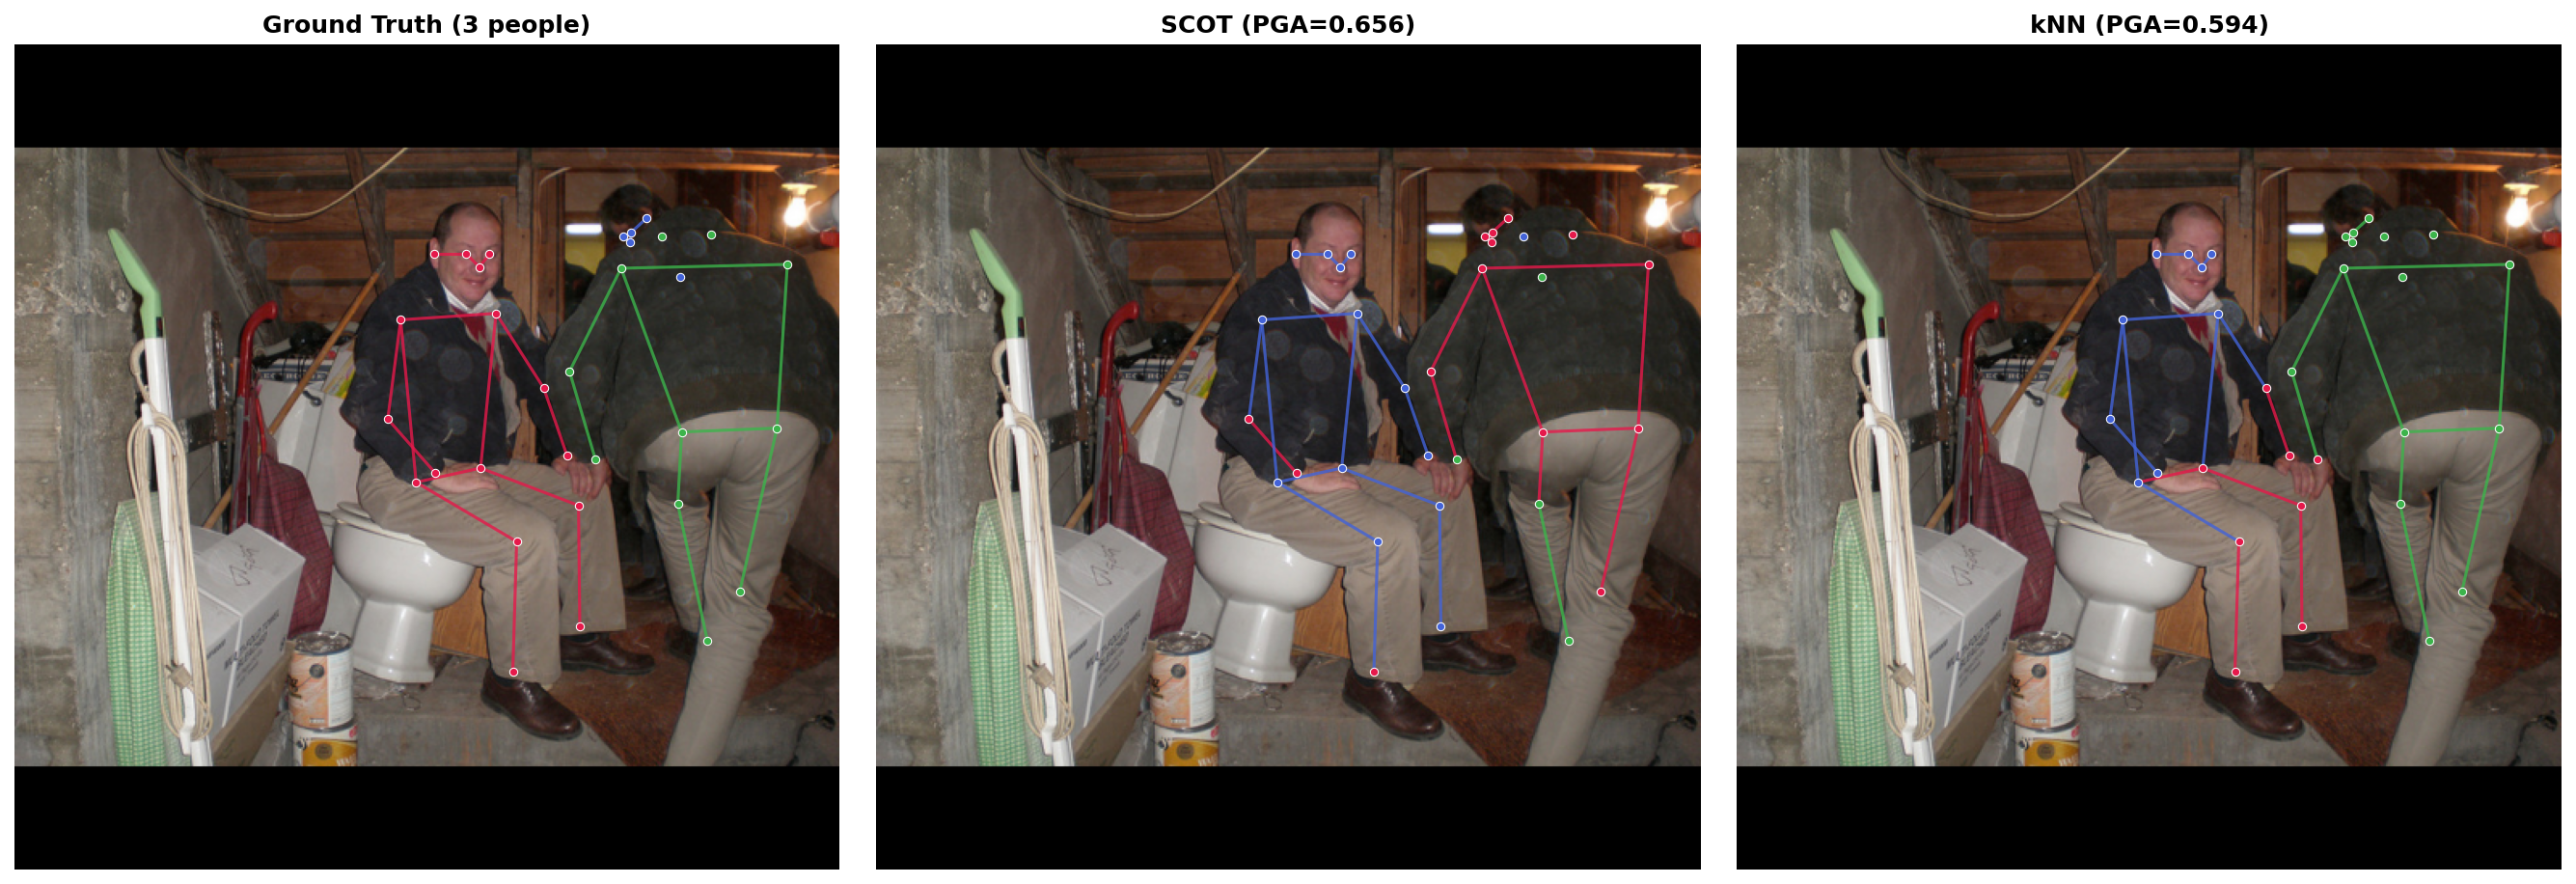
\includegraphics[width=0.85\linewidth]{figures/demo_example_1.png}
    % TODO(figure): replace with a 2x2 grid of representative synthetic
    %               scenes at K=2, K=3, K=4, K=5, with the 17 joint
    %               keypoints overlaid as coloured dots per person and
    %               the skeleton edges drawn as connecting lines.
    %               Goal: show the visual diversity of the synthetic
    %               distribution and the kind of multi-person overlap
    %               that the grouping stage must resolve.
    \caption{Representative scenes from the synthetic dataset
    at person counts $K \in \{2, 3, 4, 5\}$.
    Each panel shows the rendered Blender frame
    with the 17 per-person ground-truth keypoints overlaid
    and colour-coded by person identity.
    The synthetic generator controls camera pose, lighting,
    person placement, and visibility,
    and emits exact metric depth at each joint via raycast,
    which the depth-removal analysis of Section~\ref{sec_meth_data_depth} subsequently discards.}
    \label{fig:synth_examples}
\end{figure}

\subsection{COCO adapter}
\label{sec_meth_data_coco}

For evaluation on real images, the COCO 2017 person-keypoint annotations~\cite{lin2014coco} are loaded via the pycocotools API
and filtered to images containing at least one person.
The native COCO visibility flags ($0 = $ not labelled, $1 = $ occluded, $2 = $ visible) are mapped to the same three-value semantics as the synthetic generator.
COCO does not provide a depth channel,
so the adapter estimates one via MiDaS~\cite{ranftl2020midas},
a pre-trained monocular depth estimator that produces a per-pixel relative depth map from a single RGB image.
The DPT-Hybrid variant is used because it combines convolutional and transformer backbones and is the strongest publicly available checkpoint at moderate inference cost;
the model is instantiated once at adapter construction time
and the depth value at each labelled keypoint pixel is sampled into the $z$ slot of the keypoint vector.
This produces a $[x, y, z, v]$ representation that is dimensionally identical to the synthetic format
and that the downstream pipeline cannot distinguish from synthetic data.

The decision to estimate depth via MiDaS rather than to drop the depth channel for COCO was made
to keep the network architecture identical across data sources.
Section~\ref{sec_meth_data_depth} below describes the subsequent measurement that led to depth being removed for every method in this chapter.

\subsection{Unified pipeline}
\label{sec_meth_data_pipeline}

Both adapters emit the same per-image record:
the image tensor at $[3, H, W]$,
a list of per-person keypoint tensors at $[17, 4]$,
an image identifier,
and the person count.
A single \texttt{PoseDataset} sits behind both adapters and applies a common transform:
each image is resized to fit within $\texttt{target\_size} \times \texttt{target\_size}$ preserving aspect ratio,
symmetrically padded to the exact target dimension,
and the keypoint coordinates are scaled and shifted to match;
the $z$ and $v$ columns are passed through unchanged
and joints with $v = 0$ are not transformed at all.
A custom collate function in the dataloader stacks the image tensors but keeps the per-image keypoint lists as a list-of-lists,
because the per-image person count is variable and PyTorch's default collate cannot batch variable-length structures.

The preprocessor converts each batch into PyTorch Geometric graphs~\cite{fey2019pyg}, one graph per image.
Joints with $v = 0$ are excluded entirely from the graph rather than represented as zero-feature nodes,
so that the message passing has no spurious nodes to aggregate over.
Each surviving joint becomes a node with raw feature vector
\begin{equation}
    \mathbf{x}_i
    = [\,x_{\text{norm}},\; y_{\text{norm}},\; z_{\text{norm}},\; v_{\text{norm}}\,]
    \in \mathbb{R}^{4},
    \label{eq:node_feature_with_depth}
\end{equation}
where the spatial coordinates are normalised to $[0, 1]$ by the image dimensions,
$z_{\text{norm}}$ is a per-graph min-max normalisation of the depth over valid joints,
and $v_{\text{norm}}$ maps the three visibility levels to $\{0.0, 0.5, 1.0\}$.
The per-graph depth normalisation is what makes MiDaS-estimated COCO depth and Blender-rendered synthetic depth dimensionally compatible:
both sources land in $[0, 1]$ regardless of absolute scale.
The vector $\mathbf{x}_i$ is the raw \emph{preprocessed} feature used by the rest of the chapter;
the GAT layer-zero input $\mathbf{h}_i^{(0)}$ of Equation~\eqref{eq:layer0_input} concatenates $\mathbf{x}_i$ with the joint-type embedding.
Separate tensors per graph hold the joint-type indices (consumed by the type embedding)
and the ground-truth person labels (consumed by the contrastive loss at training time).
Edges are built by $k$-nearest neighbours in $(x_{\text{norm}}, y_{\text{norm}}, z_{\text{norm}})$ space with $k = 8$,
chosen as described in Section~\ref{sec_meth_problem_graph}.

\subsection{Removing the depth channel}
\label{sec_meth_data_depth}

The depth channel was removed from every method reported in the headline evaluations,
on the basis of a single diagnostic experiment whose result is reported in Chapter~\ref{chap_4}.
The methodological motivation is recorded here so that the rest of the chapter can refer back to it.

With depth, $k$NN clustering on contrastive GAT embeddings reaches a synthetic-test PGA of $0.994$;
the problem is effectively solved by spatial proximity in three dimensions.
The metric depth produced by the Blender renderer is exact ground truth,
so two people standing at different camera distances are separated by the $z$ coordinate alone,
and the GAT has very little discriminative work to do.
This artificially inflated all synthetic baselines and left no room for the learned heads or for SA-DMoN to demonstrate added value:
any small improvement on a near-perfect baseline is statistically indistinguishable from noise.

On COCO, the depth signal comes from MiDaS rather than from ground truth.
MiDaS produces a \emph{relative} depth ordering with no metric scale,
and the per-image scale varies with the image content.
The synthetic-to-COCO domain gap is therefore amplified by the $z$ channel:
a synthetic model trained on metric depth has learned to read $z$ at a scale that does not exist in the MiDaS output.
Removing depth removes this domain-gap component
and forces every method in this chapter to operate on the same two-dimensional signal that a real bottom-up pipeline has access to without an external depth estimator.

The removal is implemented via a \texttt{use\_depth} flag in the preprocessor configuration.
When the flag is off,
the raw feature vector of Equation~\eqref{eq:node_feature_with_depth} reduces to
\begin{equation}
    \mathbf{x}_i
    = [\,x_{\text{norm}},\; y_{\text{norm}},\; v_{\text{norm}}\,]
    \in \mathbb{R}^{3},
    \label{eq:node_feature_no_depth}
\end{equation}
the $k$NN graph is built on $(x_{\text{norm}}, y_{\text{norm}})$ only,
and the input dimension of the GAT first layer is reduced accordingly via Equation~\eqref{eq:layer0_input}.
Every result reported in Chapter~\ref{chap_4} from the baseline kNN onward uses this no-depth configuration,
unless the row is explicitly labelled as a depth-on diagnostic.
